\documentclass[twocolumn, fontsize=10pt]{article}
\usepackage[margin=0.70in]{geometry}
\usepackage{lipsum,mwe,abstract}
\usepackage[T1]{fontenc}
\usepackage[english]{babel}

\usepackage{fancyhdr} % Custom headers and footers
\pagestyle{fancyplain} % Makes all pages in the document conform to the custom headers and footers
\fancyhead{}
\fancyfoot[C]{\thepage} % Page numbering for right footer
\usepackage{lipsum}
\setlength\parindent{0pt}

\usepackage{amsmath,amsfonts,amsthm} % Math packages
\usepackage{wrapfig}
\usepackage{graphicx}
\usepackage{float}
\usepackage{subcaption}
\usepackage{comment}
\usepackage{enumitem}
\usepackage{cuted}
\usepackage{sectsty} % Allows customizing section commands
\allsectionsfont{\normalfont \normalsize \scshape} % Section names in small caps and normal fonts

\renewenvironment{abstract} % Change how the abstract look to remove margins
 {\small
  \begin{center}
  \bfseries \abstractname\vspace{-.5em}\vspace{0pt}
  \end{center}
  \list{}{%
    \setlength{\leftmargin}{0mm}
    \setlength{\rightmargin}{\leftmargin}%
  }
  \item\relax}
 {\endlist}

\makeatletter
\renewcommand{\maketitle}{\bgroup\setlength{\parindent}{0pt} % Change how the title looks like
\begin{flushleft}
  \textbf{\@title}
  \@author \\
  \@date
\end{flushleft}\egroup
}
\makeatother

%% -------------------------------------------------------------------

\title{
\Large X-Ray threat detection \\
[10pt]
}
\date{September 1, 2024}
\author{Riccardo Inverardi Galli}

\begin{document}

\twocolumn[ \maketitle ]

% --------------- ABSTRACT
\begin{abstract}
    The scope of this project was to create a convolutional neural network designed to detect dangerous items in X-ray luggage scans. A combination of convolutional layers, batch normalization, and linear activations was employed to achieve this goal. The model was trained on a dataset containing both dangerous and potentially dangerous items. To improve the model's ability to detect general features across different classes, the dataset was augmented using random rotations and random cropping, resulting in over 15,000 images across 8 different classes. After 60 epochs of training, the model performs well on the validation set, achieving at least 0.90 accuracy in every class. These results were consistent across different training/validation splits, indicating that it possessses ability to generalize. The model was developed exclusively using Python's PyTorch library.
\end{abstract}

\rule{\linewidth}{0.5pt}

% --------------- MAIN CONTENT

% If you want to put a big figure over two columns, you can use \begin{figure*}
% The figure will be sent on top of the next page


\begin{figure*}
    \centering
    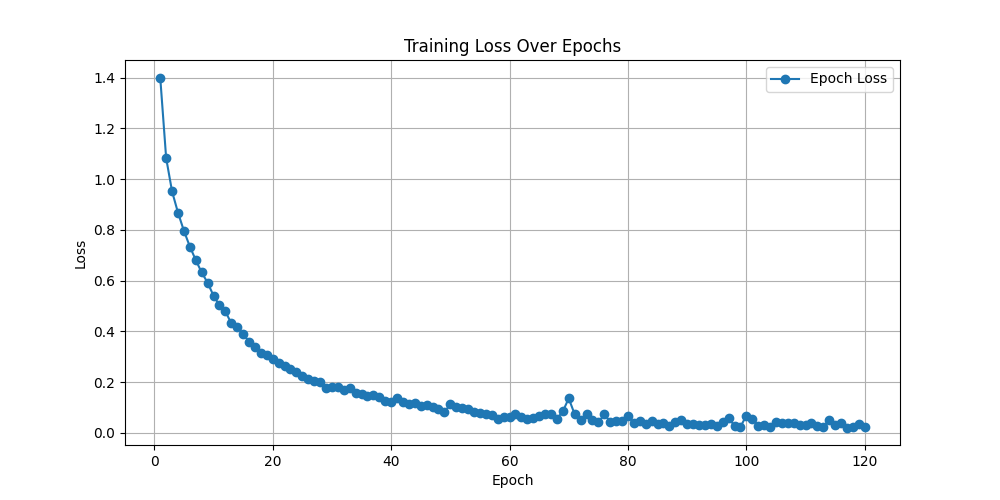
\includegraphics[width=0.9\textwidth]{loss_function.png}
    \caption{Loss function value}
\end{figure*}
% You can also use the following command, but it can be more tricky to place the figure exactly where you want
% \begin{strip}
%     \centering\noindent
%     \includegraphics[width=0.9\textwidth]{Dummy_fig.png}
%     \captionof{figure}{Caption}
% \end{strip}


\section{Introduction}
 In commercial aviation, the security of crew members and passengers has always been a major concern. X-ray scans have long played a crucial role in ensuring passenger safety, and the use of machine learning in this field is growing rapidly. While it is still early to consider replacing human supervision with automated systems, a reliable threat detection model could greatly assist human operators, who are naturally prone to error or may be misled by complex images. The goal of this model, though still in early development, is to provide support in situations where the human eye might be deceived. The model was trained on a dataset containing images of luggage with eight different classes of dangerous items: cameras, cellphones, various electronic devices, knives, laptops, lighters, power banks, and scissors. Currently, it is only trained on classes that contain dangerous items and does not yet have the ability to recognize non-dangerous luggage.

\section{The model - Preprocessing step}
The model is built as a subclass of PyTorch's nn.Module class. It contains two preprocessing layers that perform gaussian blur and edge detection by applying 3x3 convolutions with the following kernels.

\[
\overset{\text{Gaussian Blur}}{\begin{bmatrix}
1 & 2 & 1 \\
2 & 4 & 2 \\
1 & 2 & 1
\end{bmatrix}
}
\quad
\overset{\text{Edge Detection}}{\begin{bmatrix}
0 & -1 & 0 \\
-1 & 4 & -1 \\
0 & -1 & 0
\end{bmatrix}
}
\]

This helps in getting rid of unnecessary noise during training, so that the model only focuses on the actual luggage, discarding any background.

\section{Convolutional Blocks and Fully Connected Layers}
The first convolutional block expands the preprocessed images to 32 channels. Padding is applied to prevent the reduction of image dimensions due to the convolution's effect on border pixels. Following this, batch normalization is performed, and the output is passed through the hyperbolic tangent activation function. Finally, a max-pooling operation with a \(2 \times 2\) window is applied. The hyperbolic tangent activation function, denoted as \(\tanh(x)\), is defined as:

\[
\tanh(x) = \frac{e^x - e^{-x}}{e^x + e^{-x}}
\]

The same convolution is again repeated in the second block, reducing the number of output channels from 32 to 16. The final linear layers take the flattened output of the convolutional blocks and map it to 32 and then 8 dimensional input, reprensenting the 8 classes of the model.

\section{The Pipeline}
The model is trained through a pipeline that covers all essential steps for training. Initially, images are loaded, resized to 64x64 pixels, and converted into tensors. The dataset is then split into training and validation sets using a custom splitting function, ensuring that validation is conducted on a separate subset of data, which helps prevent overfitting. Images belonging to the same class are stacked together to facilitate efficient batch processing. At this stage, normalization is performed independently on each class on both the training and validation sets to standardize the data. The normalized images are subsequently formatted, each image tensor is paired with its corresponding class label and organized into a flat list of tuples. Data loaders for both the training and validation sets are created using torch.utils.data.DataLoader, with a batch size of 64. To perform gradient descent over the loss function, Stochastic Gradient Descent (SGD) is employed for optimizing the model, where the true gradient of the loss function is approximated using the gradient at a single sample. The model parameters are updated based on this approximated gradient, weighted by the learning rate, as described by the equation:

\[
\theta := \theta + \alpha(y_i - h_{\theta}(x_i))x_i
\]

Here, \(h_{\theta}(x_i)\) represents the predicted value for sample \(x_i\), \(y_i\) is the ground truth label, and \(\alpha\) is the learning rate. Cross Entropy Loss is used as the loss function, chosen to avoid the need for combining LogSoftMax with Negative Log Likelihood Loss, thus simplifying the loss computation. L2 regularization is applied to the training loop by setting the weight decay parameter in the optimizer (SGD) object. This ensures that the model is less prone to overfitting. By training the model for more epochs, we see that the behaviour of the loss function using SGD tends to a global minimum after 80/90 epochs of training.

\begin{figure}[htb]
\centering
\includegraphics[width=0.9\textwidth]{model.parameters.png}
\caption{The model}
\end{figure}

\section{Conclusion}
Altough this model is still in the early stages of its development, it showcases the full power of convolutions, making inference possible over complex images while keeping the number of parameters in check. With an accuracy exceeding 0.98 across all classes on the validation set, the model shows strong generalization capabilities and reliability. Although still in early stages, it provides a valuable tool to support human operators in identifying potential threats, ultimately aiming to improve safety and efficiency in the security screening process. Future work will focus on expanding the model’s capabilities to recognize non-dangerous items and integrating it into real-world screening systems.


%\begin{thebibliography}{}
%\bibitem{Ref1}{First reference}
%\bibitem{Ref2}{Second reference}
%\bibitem{Ref3}{Third reference}
%\end{thebibliography}


 \end{document}
